\section{Einheitssignale}
	
	\subsection{Funktionen}
	\renewcommand{\arraystretchOriginal}{1}
	\begin{tabular}{ll}
		\textbf{Sprungfunktion \skript{16}} &
		Einschaltfunktion, Einheitssprung, Heaviside-Function \matlab{heaviside}
		\\
		\parbox{6cm}{
			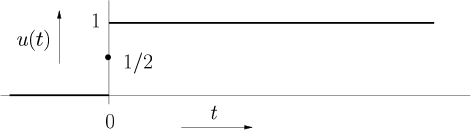
\includegraphics[width=5.5cm]{./bilder/sprungfunktion.png}
		}
		&
		\parbox{12cm}{
			$$u(t) = 1(t) = 
  			\begin{cases}
    			0 & \mbox{f"ur } t < 0,\\
    			\frac{1}{2} & \mbox{f"ur } t = 0,\\
    			1 & \mbox{f"ur } t > 0.\\
  			\end{cases}$$	
			$$\mathcal{L:}\quad u(t) \; \laplace \; \frac1s$$
		}
		\\ \hline & \\
		
		\textbf{Signumfunktion \skript{16}} &
		Vorzeichenfunktion \matlab{sign}
		\\
		\parbox{6cm}{
			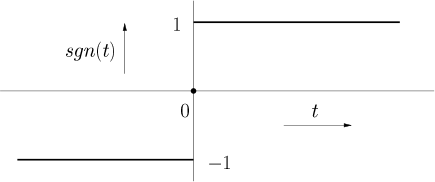
\includegraphics[width=5.5cm]{./bilder/sign.png}
		}
		&
		\parbox{12cm}{
			$$\sgn(t) =
  			\begin{cases}
    			-1 & \mbox{f"ur } t < 0,\\
    			0 & \mbox{f"ur } t = 0,\\
    			1 & \mbox{f"ur } t > 0.\\
  			\end{cases}$$
			$$\mathcal{F:}\quad \sgn(t) \; \laplace \; \frac{-2j}{\omega}$$ \\
		}
		\\ \hline & \\

		\textbf{Rampenfunktion \skript{17}} & \matlab{ramp}
		\\
		\parbox{6cm}{
			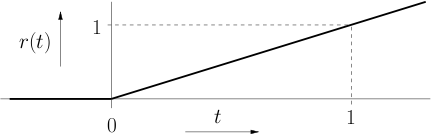
\includegraphics[width=5.5cm]{./bilder/ramp.png}
		}
		&
		\parbox{12cm}{
			$$r(t) = t u(t) =
  			\begin{cases}
    			0 & \mbox{f"ur } t \leq 0\\
    			t & \mbox{f"ur } t > 0\\
  			\end{cases}$$
			$$\mathcal{L:}\quad r(t) \; \laplace \; \frac{1}{s^2}$$ \\
		}
		\\ 
		\end{tabular}
		
		\begin{tabular}{ll}
		\textbf{Rechteckimpuls \skript{17}} & 
		\\
		\parbox{6cm}{
			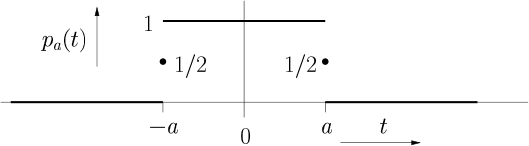
\includegraphics[width=5.5cm]{./bilder/rechteckimpuls.png}
		}
		&
		\parbox{12cm}{
			$$p_a(t) = u(t+a) -u(t-a) = 
  			\begin{cases}
    			1 & \mbox{f"ur } |t| < a\\
    			\frac{1}{2} & \mbox{f"ur } |t| = a\\
    			0 & \mbox{f"ur } |t| > a\\
  			\end{cases}$$
			$$\mathcal{F:}\quad p_a(t) \; \laplace \; 2a \sinc(a \omega) = \frac{2}{\omega} \sin(a \omega)$$ \\
		}
		\\ \hline & \\

		\textbf{Dreieckimpuls \skript{18}} & 
		\\
		\parbox{6cm}{
			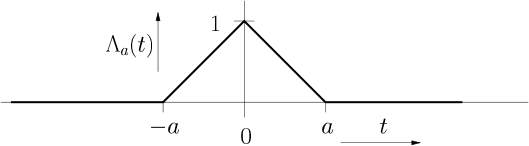
\includegraphics[width=5.5cm]{./bilder/dreieckimpuls.png}
		}
		&
		\parbox{12cm}{
			$$\Lambda_a(t) =
  			\begin{cases}
    			1 - \frac{|t|}{a}& \mbox{f"ur } |t| < a\\
    			0 & \mbox{f"ur } |t| \geq a\\
  			\end{cases}$$
			$$\mathcal{F:}\quad \Lambda_a(t) \; \laplace \;
			a\left(\frac{\sin(\frac{a\omega}{2})}{\frac{a\omega}{2}}\right)^2 = a \sinc^2\left(\frac{a\omega}{2}\right)$$ \\
		}
		\\ \hline & \\

		\textbf{Sincfunktion \skript{18}} &
		\matlab{sinc}
		\\
		\parbox{6cm}{
			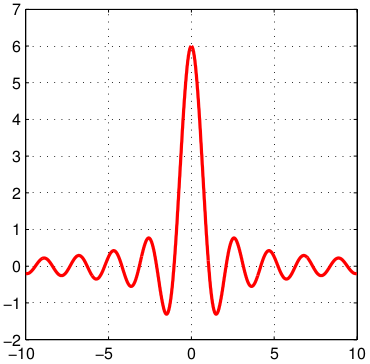
\includegraphics[width=5.5cm]{./bilder/sinc.png}
		}
		&
		\parbox{12cm}{
			$$ \sinc_{\alpha}(t) = \frac{\sin(\alpha t)}{t} \qquad 
			\sinc(\alpha t) = \frac{\sin(\alpha t)}{\alpha t}$$
			$$\mathcal{F:}\quad  \sinc_{\alpha}(t) = \frac{\sin(\alpha t)}{t} \; \laplace \;
			\pi p_{\alpha}(\omega)$$
			$$\mathcal{F:}\quad  \sinc(\alpha t) = \frac{\sin(\alpha t)}{\alpha t} \; \laplace \;
			\frac{\pi}{\alpha} p_{\alpha}(\omega)$$ } \\
		\end{tabular}

		\begin{tabular}{ll}
		\textbf{Impulsfunktion \skript{19}} &
		Diracimpuls, Diracstoss, Deltaimpuls \matlab{dirac}
		\\
		\parbox{5cm}{
			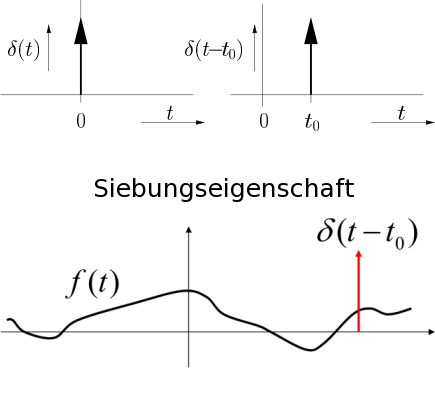
\includegraphics[width=5cm]{./bilder/dirac.png}
		}
		&
		\parbox{13cm}{
			$$\delta(t) =
  			\begin{cases}
    			\infty & \mbox{f"ur } t = 0\\
    			0 & \mbox{sonst}\\
  			\end{cases}$$
		\begin{tabular}{|r|c|l|} \hline
	 		1. & $\delta(at) = \frac{1}{|a|}\delta(t)$ & Skalierung\index{Skalierung}\\ \hline
	 		2. & $\delta(\frac{t-t_0}{a}) = |a|\cdot\delta(t-t_0)$ & Skalierung und Verschiebung  \\ \hline
	 		3. & $\delta(-t+t_0) = \delta(t-t_0)$ & symmetrisch\\ \hline
	 		4. & $\delta(-t) = \delta(t)$ & $\delta(t)=\mbox{ gerade Funktion}$ \\ \hline
	 		\textbf{5.} & $\int\limits_{-\infty}^{\infty}\delta(t-t_0)f(t)dt = f(t_0)$ & \textbf{Siebungseigenschaft}\\ \hline
	 		6. & $\delta(t-t_0)f(t) = f(t_0)\delta(t-t_0)$ &  Abtastung\index{Abtastung}\\ \hline
	 		\textbf{7.} & $\int\limits_{-\infty}^{\infty}A\cdot\delta(t)dt = A$ & \textbf{Spezialfall der Siebungseigenschaft} \\ \hline
	 		8. & $\delta(t-t_0)\ast f(t) = f(t-t_0)$ & Faltung\\ \hline
	 		9. & $\delta(t-t_1)\ast\delta(t-t_2) = \delta(t-t_1-t_2)$ & Faltung\index{Faltung}\\ \hline
			10. & $\delta(t)=\frac{\partial u(t)}{\partial t}$ & Ableitung des Einheitssprungs\index{Ableitung}\\ \hline
			11. & $\delta(t)=\lim\limits_{\omega\rightarrow \infty}\frac{\sin(\omega t)}{\pi t}$ & Definition\\ \hline 
			12. & $\mathcal{L}, \mathcal{F}:\quad \delta(t) \; \laplace \; 1$ 
			& Frequenzbereich
		\\ \hline
		\end{tabular}
		\\
		\vspace{.1cm}\\
		}
		\end{tabular}

	

	\begin{sidewaystable}
\subsection{Eigenschaften unterschiedlicher Schwingungsformen}
\begin{center}
\begin{tabular}{|l|c|c|c|c|c|c|c|c|}
\hline
	Schwingungsform & Funktion & Gleichrichtwert & Formfaktor &
	Effektivwert & Scheitelfaktor & \textbf{$X_0$} & \textbf{$X^2$} & \textbf{var(X)} \\
\hline
	Formel &
	&
	$\overline{\left|x\right|} = \frac1T\int_{0}^{T}\left| x(t)\right|dt$&
	$\frac{X}{\overline{\left|x\right|}}$&
	$X = \sqrt{X^2} = \sqrt{\frac{1}{T} \int\limits ^{t_0+T}_{t_0}{x^2(t)dt}}$&
	$k_{s}=\frac{X_{\mathrm{max}}}{X_{\mathrm{eff}}}$&
	&
	&
	\\
\hline
	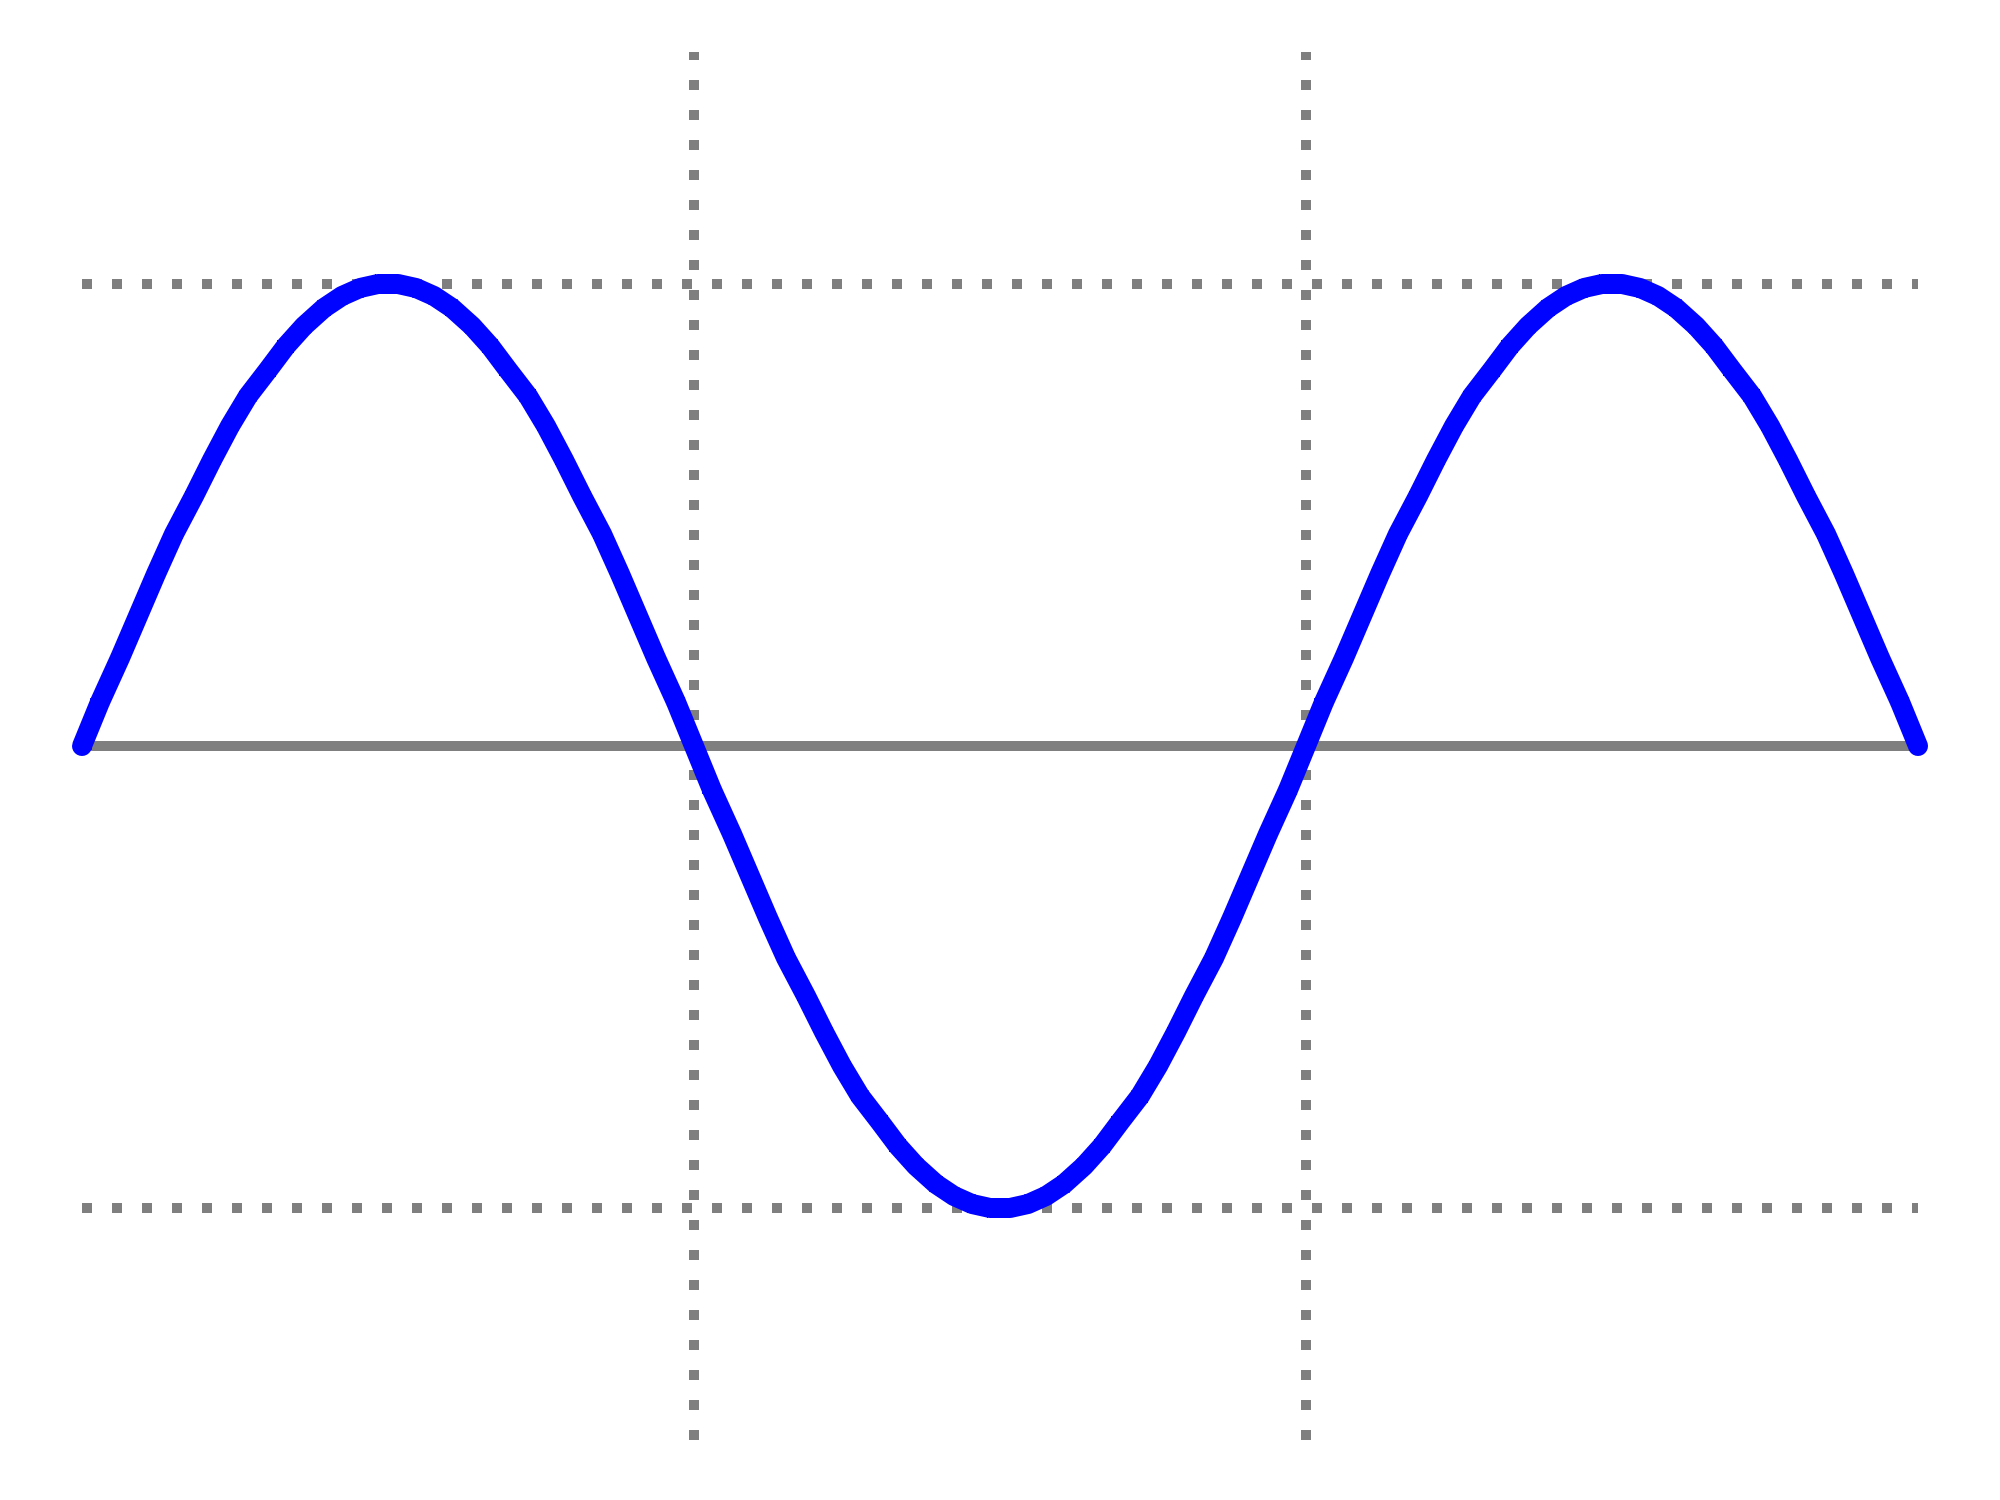
\includegraphics[width=2cm]{table/images/table_sine_wave.png} &
	$A\cdot\sin(t)$ &
	$\frac{2}{\pi} \approx 0.637$ &
	$\frac{\pi}{2\sqrt{2}} \approx 1.11$ &
	$\frac{1}{\sqrt{2}}\approx 0.707$ &
	$\sqrt{2}\approx 1.414$ &
	$0$ &
	$\frac{A^2}{2}$ &
	$\frac{A^2}{2}$ \\
\hline	
	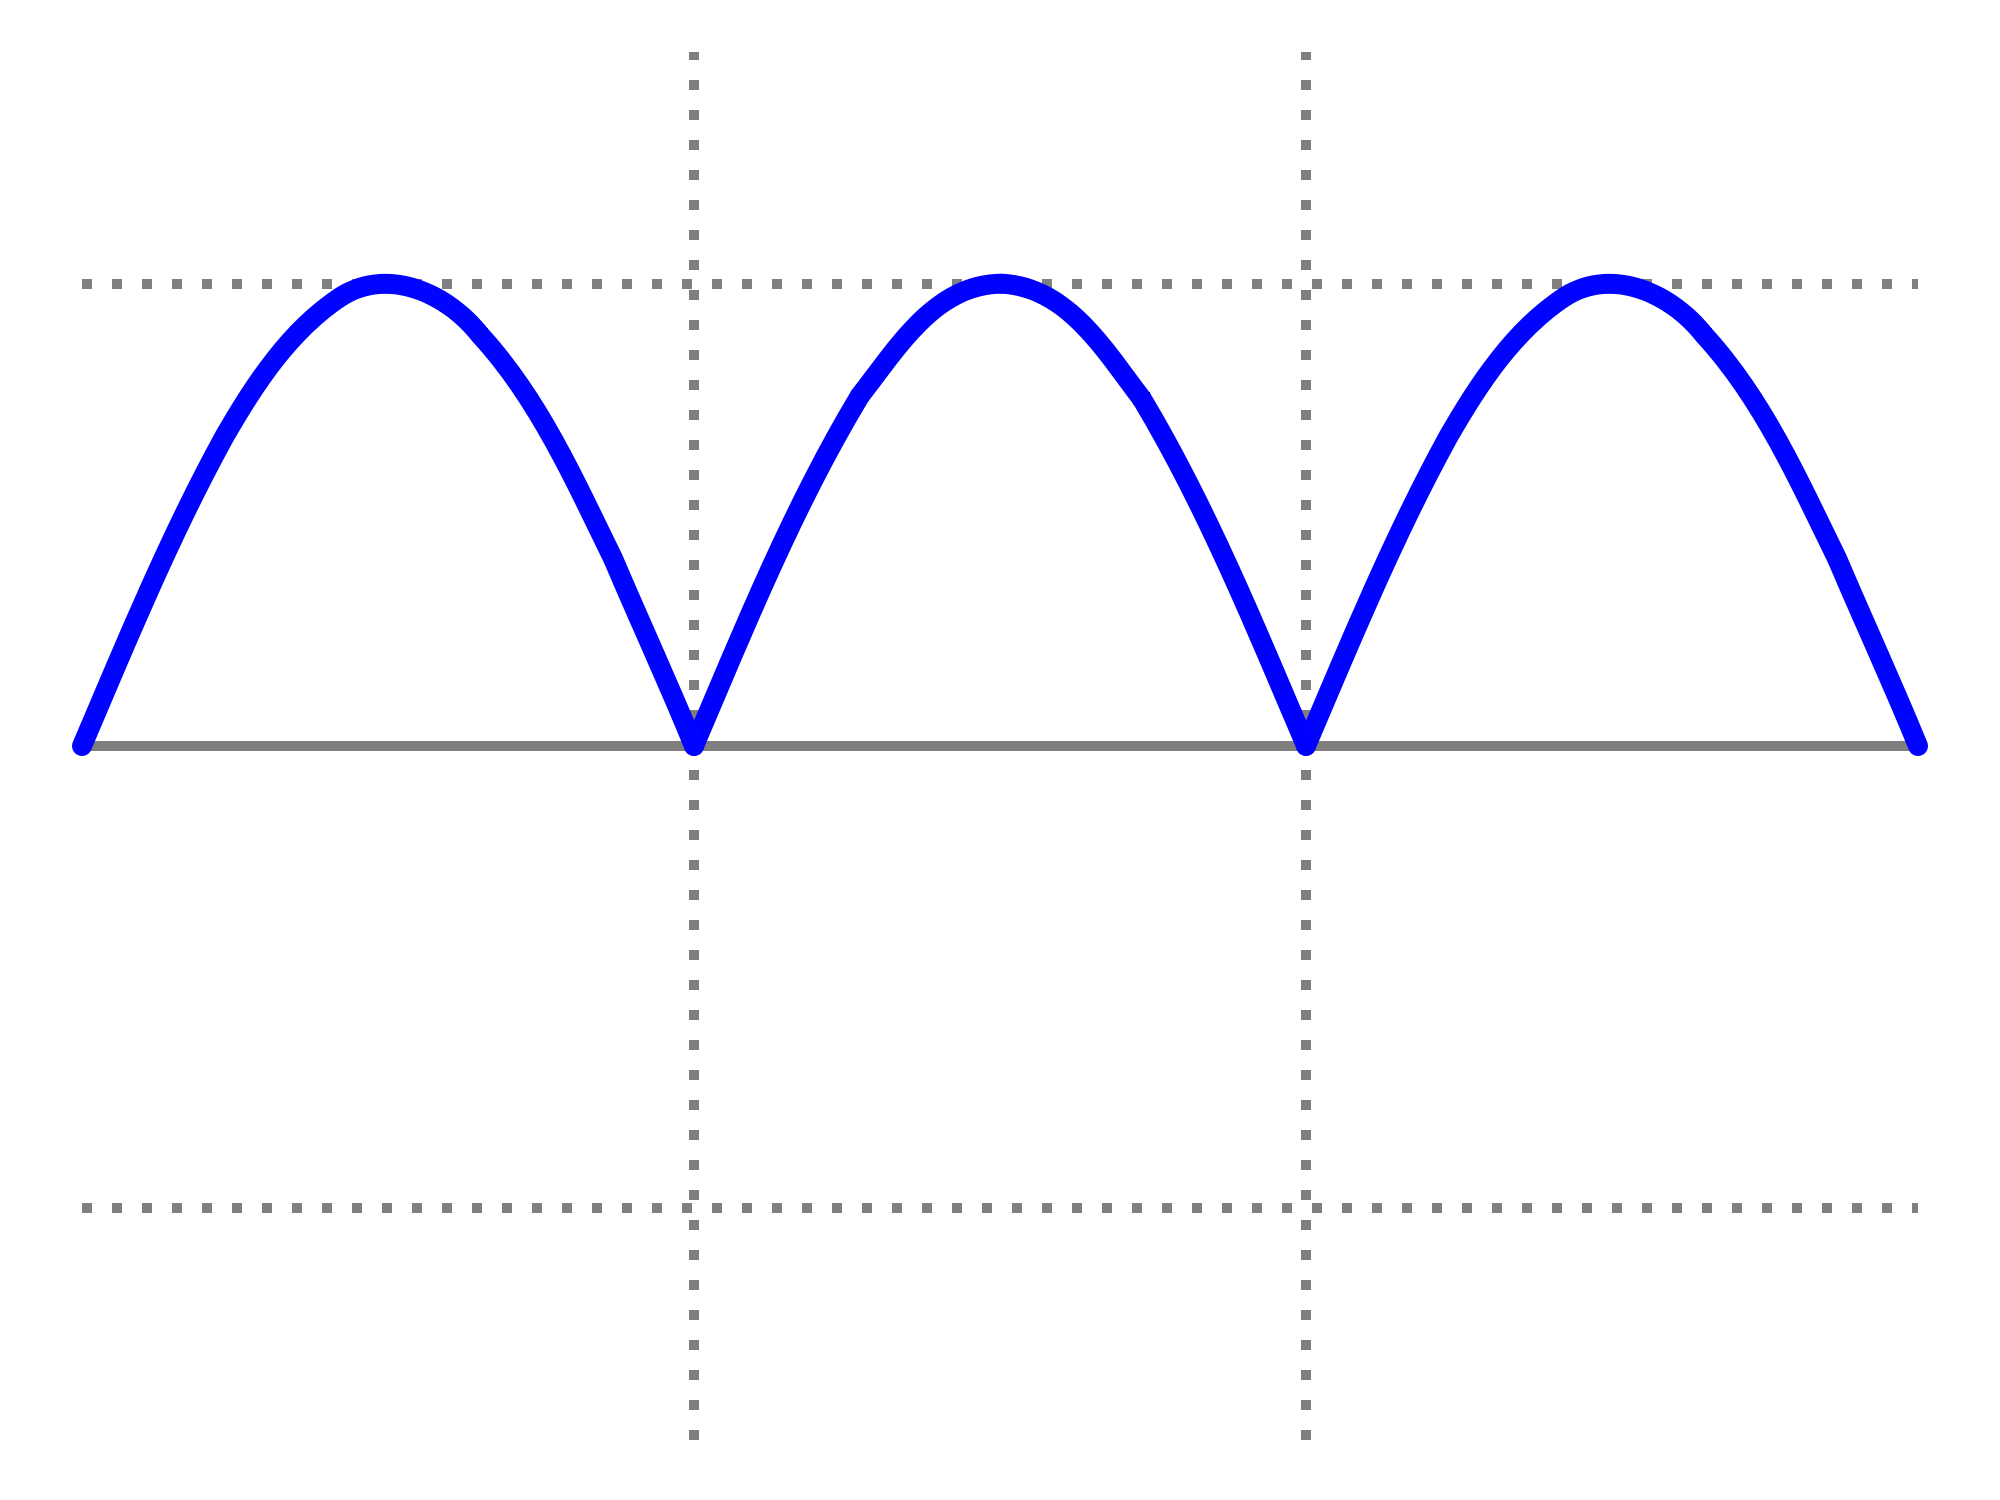
\includegraphics[width=2cm]{table/images/table_full-wave_rectified_sine.png} &
	$A\cdot|\sin(t)|$ &
	$\frac{2}{\pi} \approx 0.637$ &
	$\frac{\pi}{2\sqrt{2}} \approx 1.11$ &
	$\frac{1}{\sqrt{2}} \approx 0.707$ &
	$\sqrt{2} \approx 1.414$  &
	$\frac{2A}{\pi}$ & $\frac{A^2}{2}$ & $\frac{A^2}{2}-\frac{4A^2}{\pi^2}$
	\\
\hline
	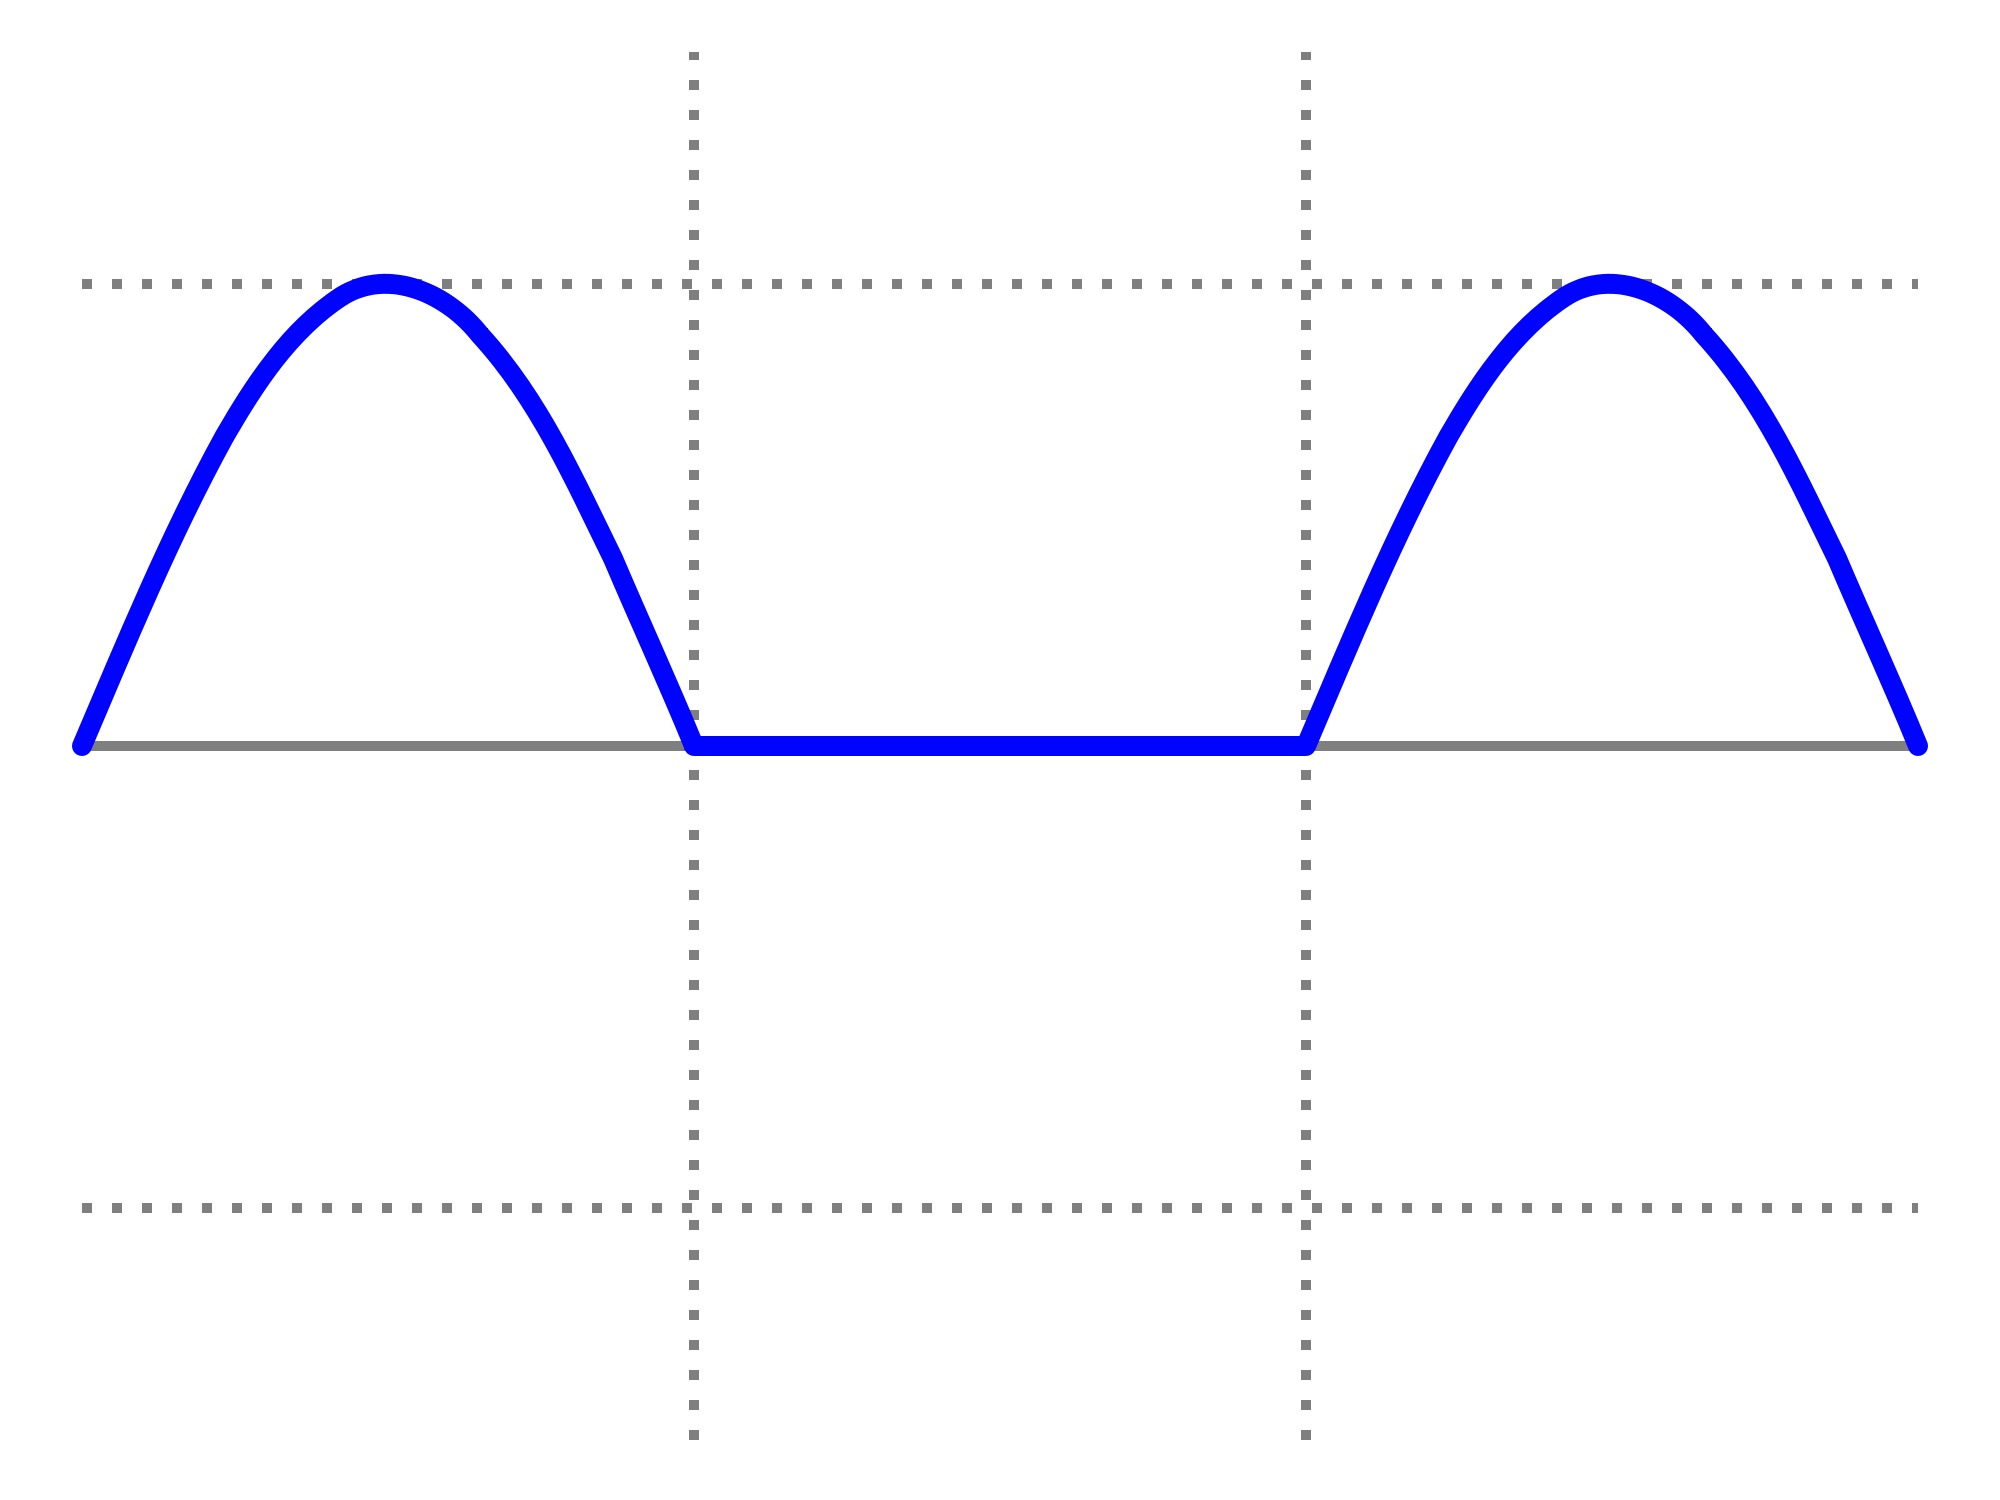
\includegraphics[width=2cm]{table/images/table_half-wave_rectified_sine.png} &
	$\begin{cases} A\cdot\sin (t) & 0<t<\pi  \\ 0 & \text{True}\end{cases}$ &
	$\frac{1}{\pi}\approx 0.318$ &
	$\frac{\pi}{2}\approx 1.571$ &
	$\frac{1}{2} = 0.5$	&
	2  &
	$\frac{A}{\pi}$ &
	$\frac{A^2}{4}$ & $\frac{A^2}{4}-\frac{A^2}{\pi^2}$
	\\
\hline
	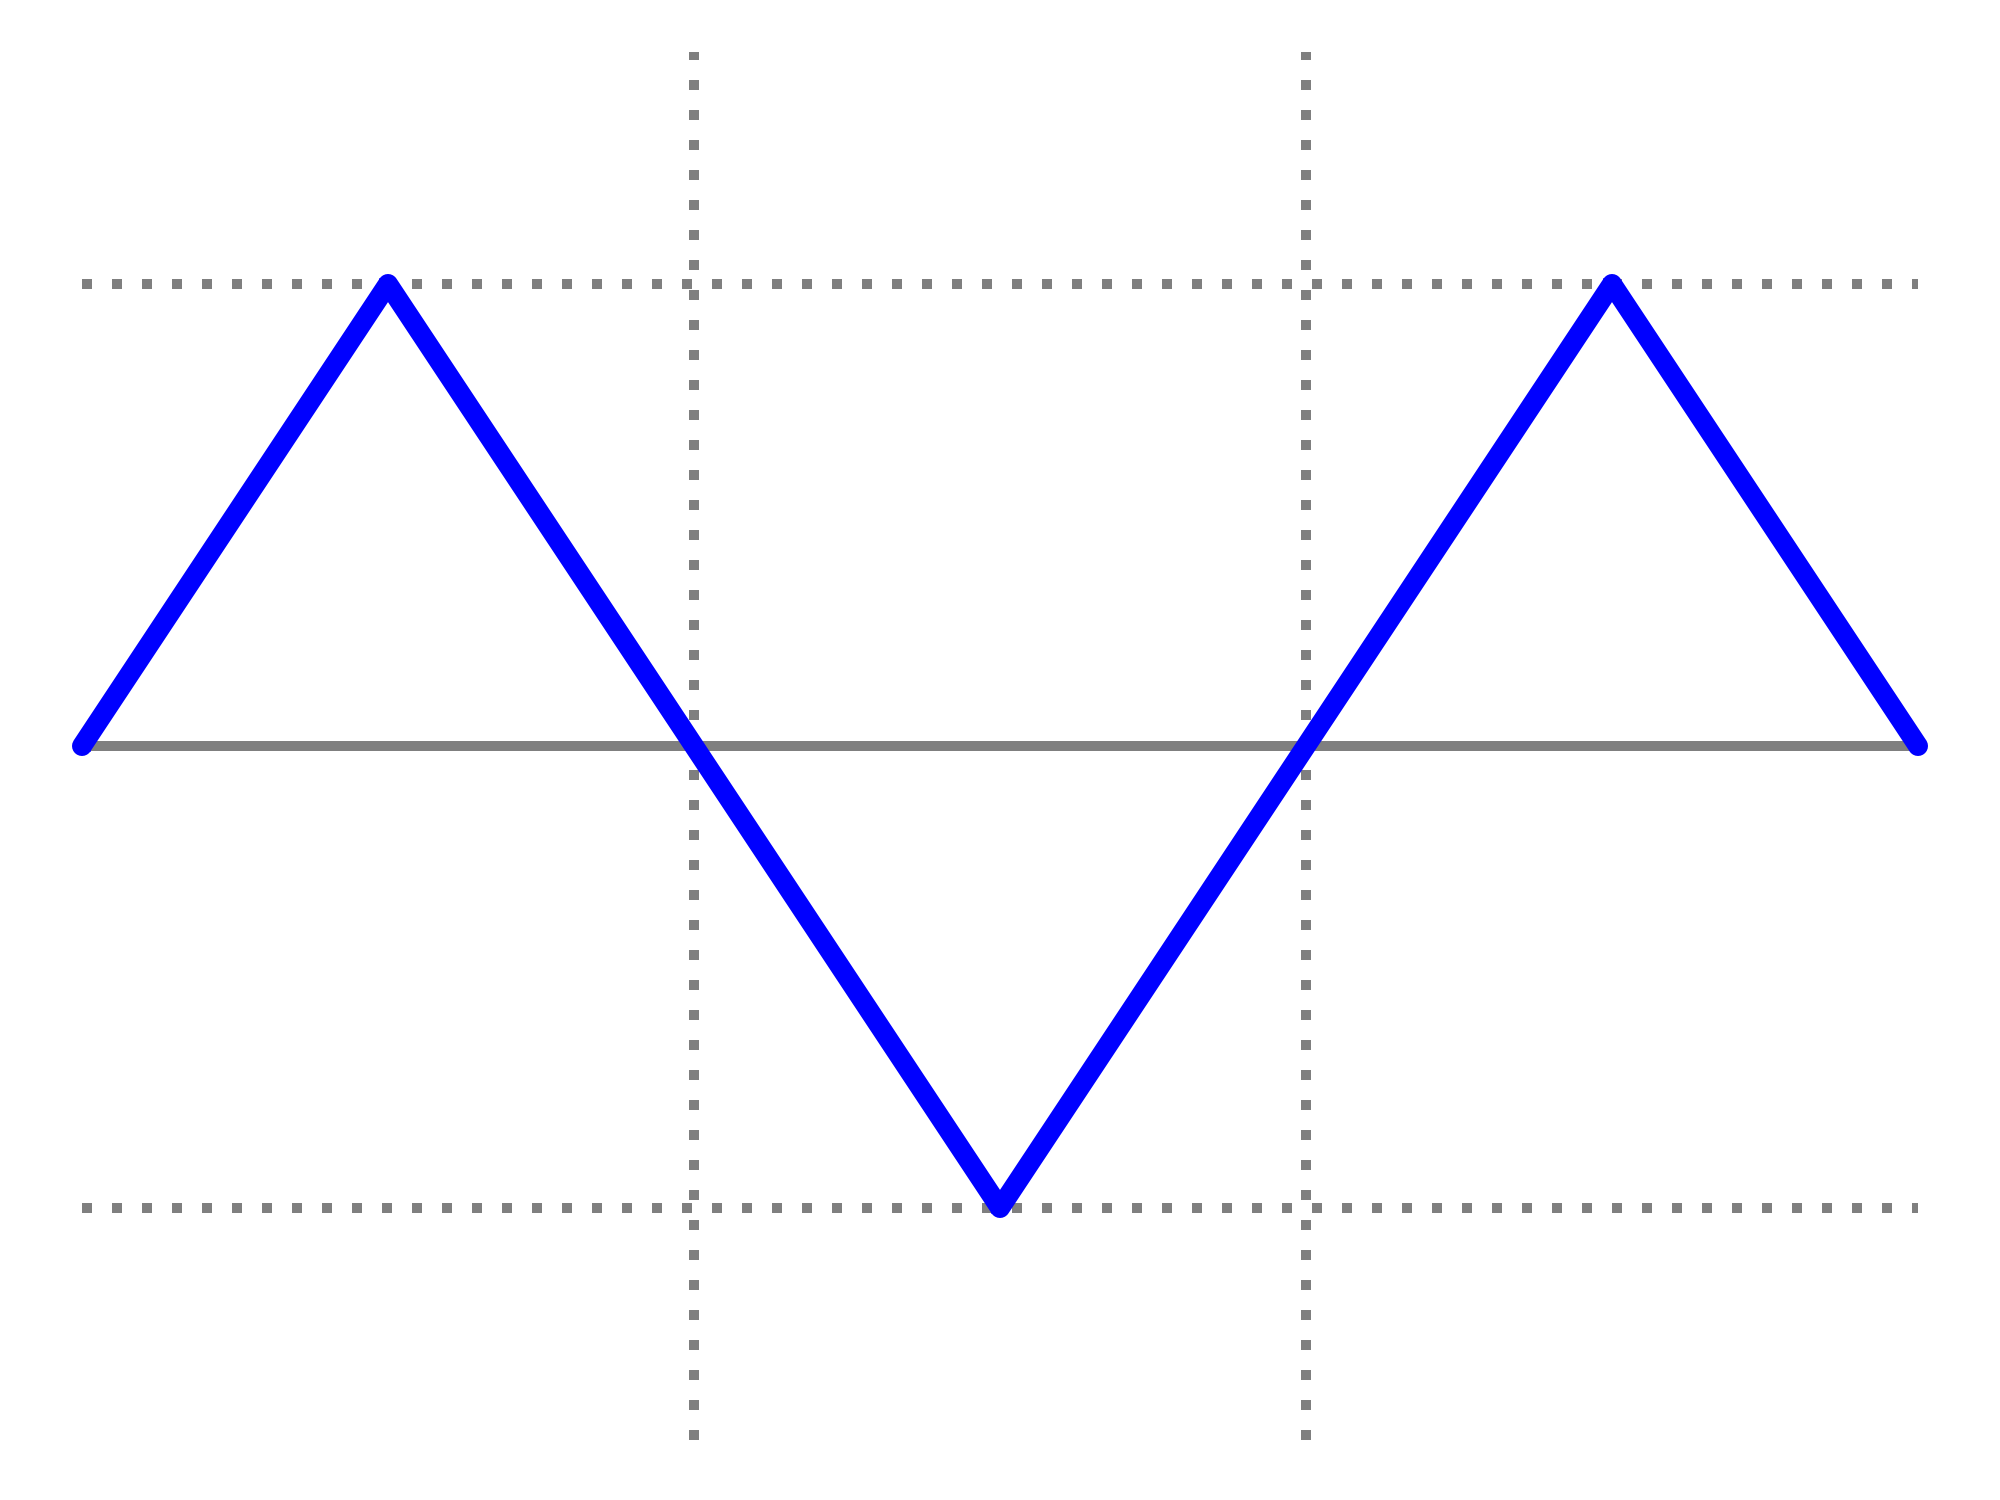
\includegraphics[width=2cm]{table/images/table_triangle_wave.png} &
	$A\cdot\Lambda(t)$ &
	$\frac{1}{2}= 0.5$ &
	$\frac{2}{\sqrt{3}}\approx 1.155$ &
	$\frac{1}{\sqrt{3}}
	\approx 0.557$ &
	$\sqrt{3} \approx 1.732$ &
	$0$ &
	$\frac{A^2}{3}$ &
	$\frac{A^2}{3}$ \\
\hline	
	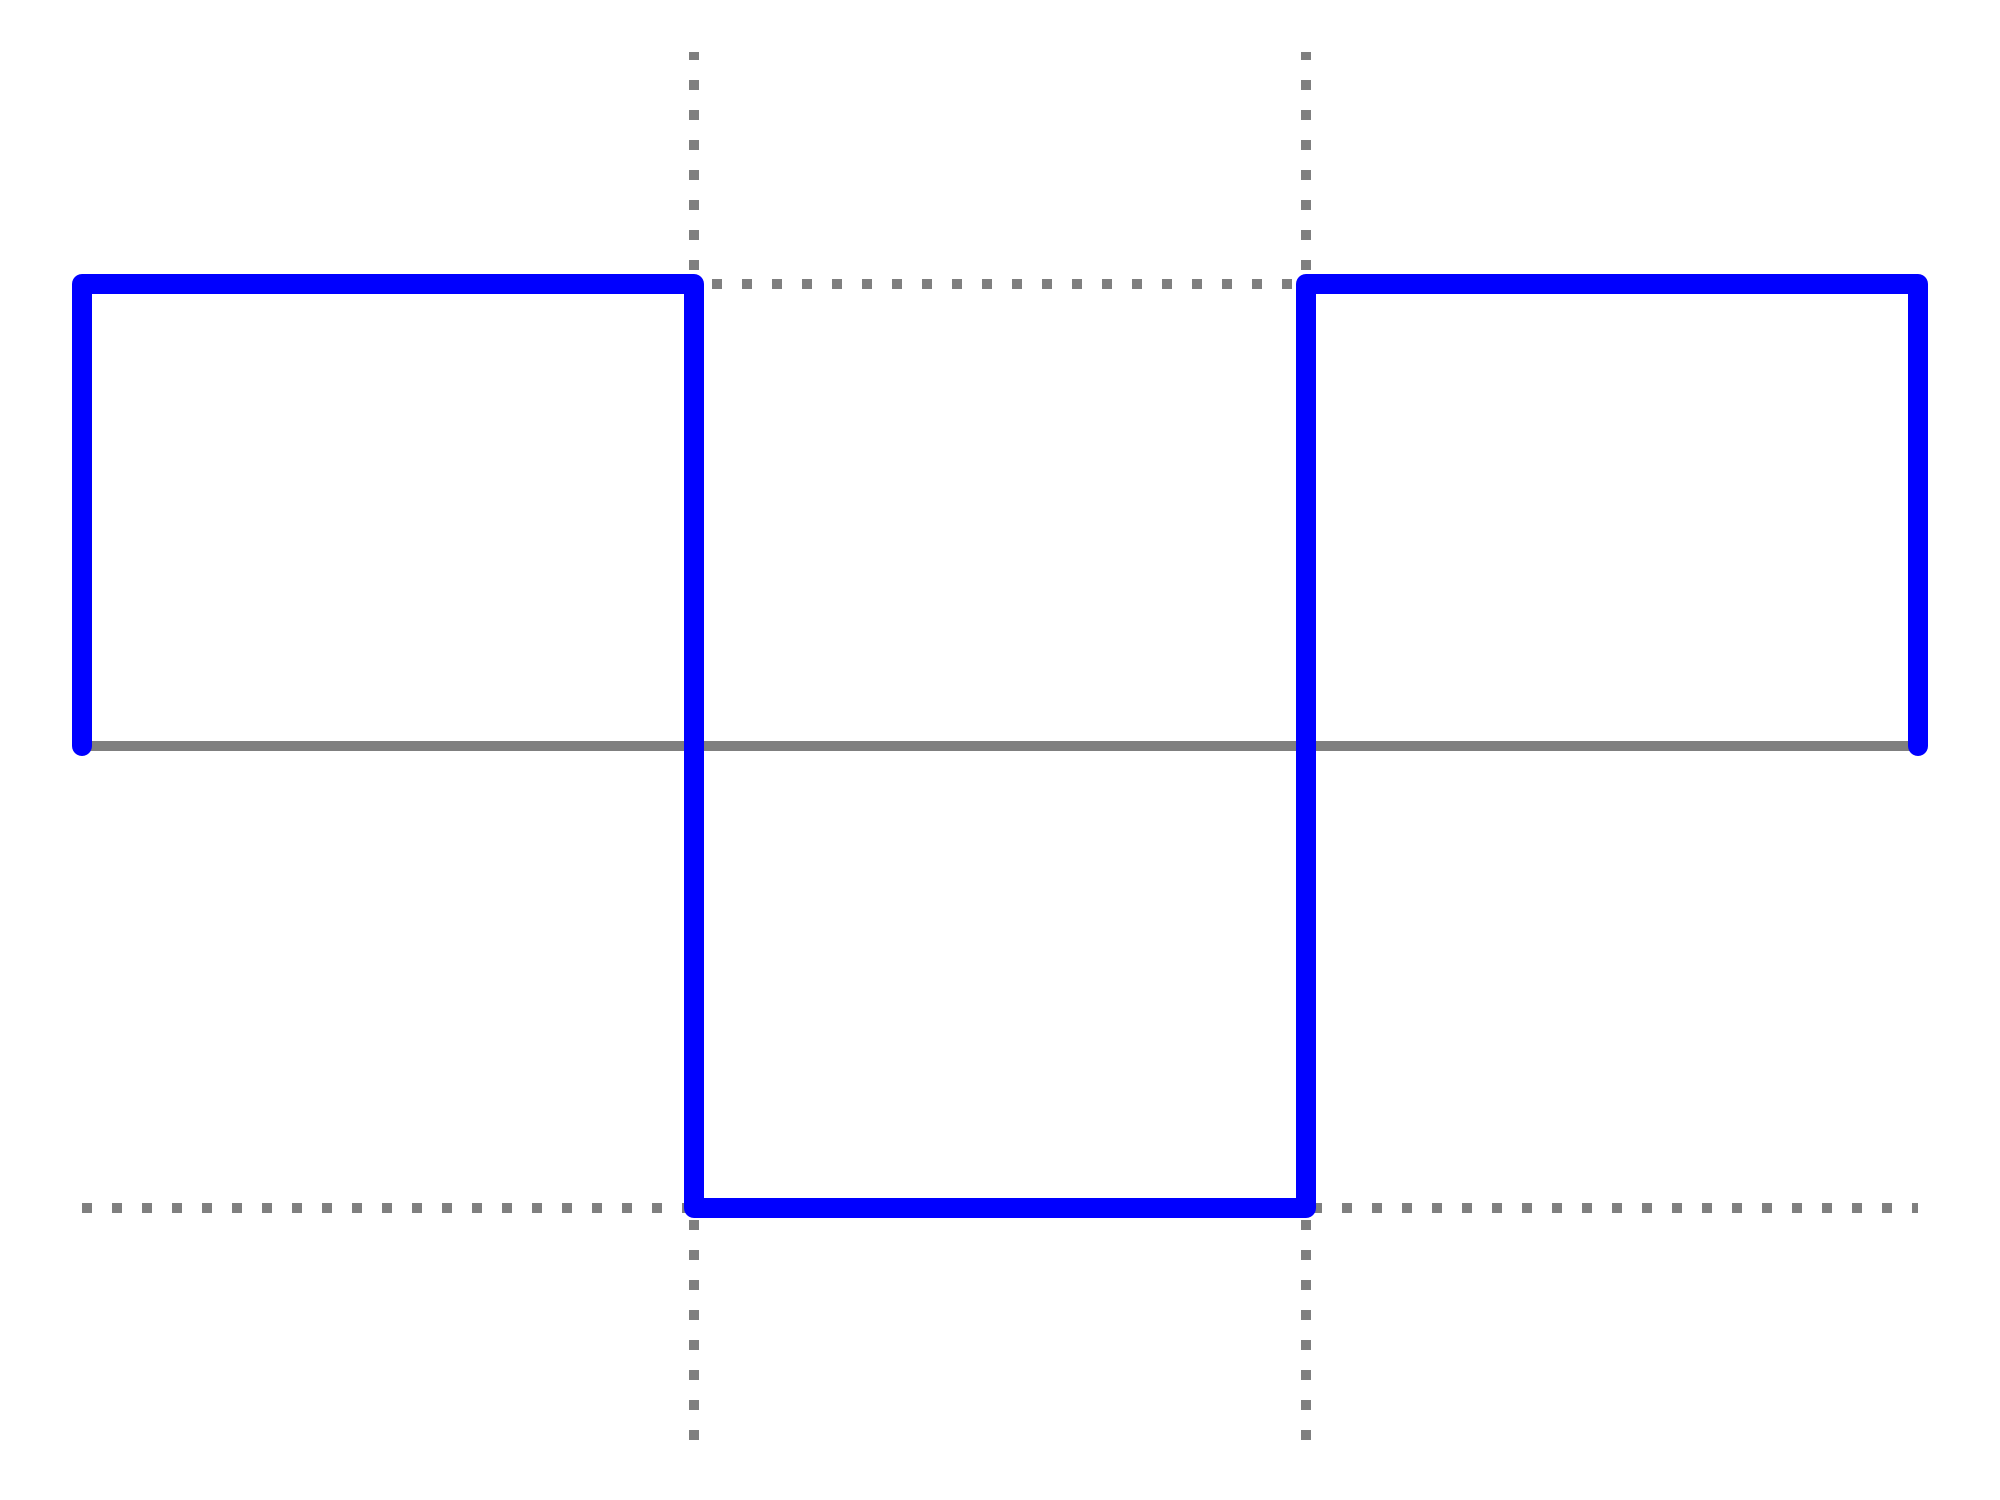
\includegraphics[width=2cm]{table/images/table_square_wave.png} &
	$\begin{cases} A & 0<x<t \\ 0 & \text{True}\end{cases}$ &
	$1$ &
	$1$ &
	$1$ &
	$1$ &
	$0$ &
	$A^2$ &
	$A^2$ \\
\hline	
	DC&
	1&
	$1$ &
	$1$ &
	$1$ &
	$1$  &
	-&
	-&
	-\\
\hline	
	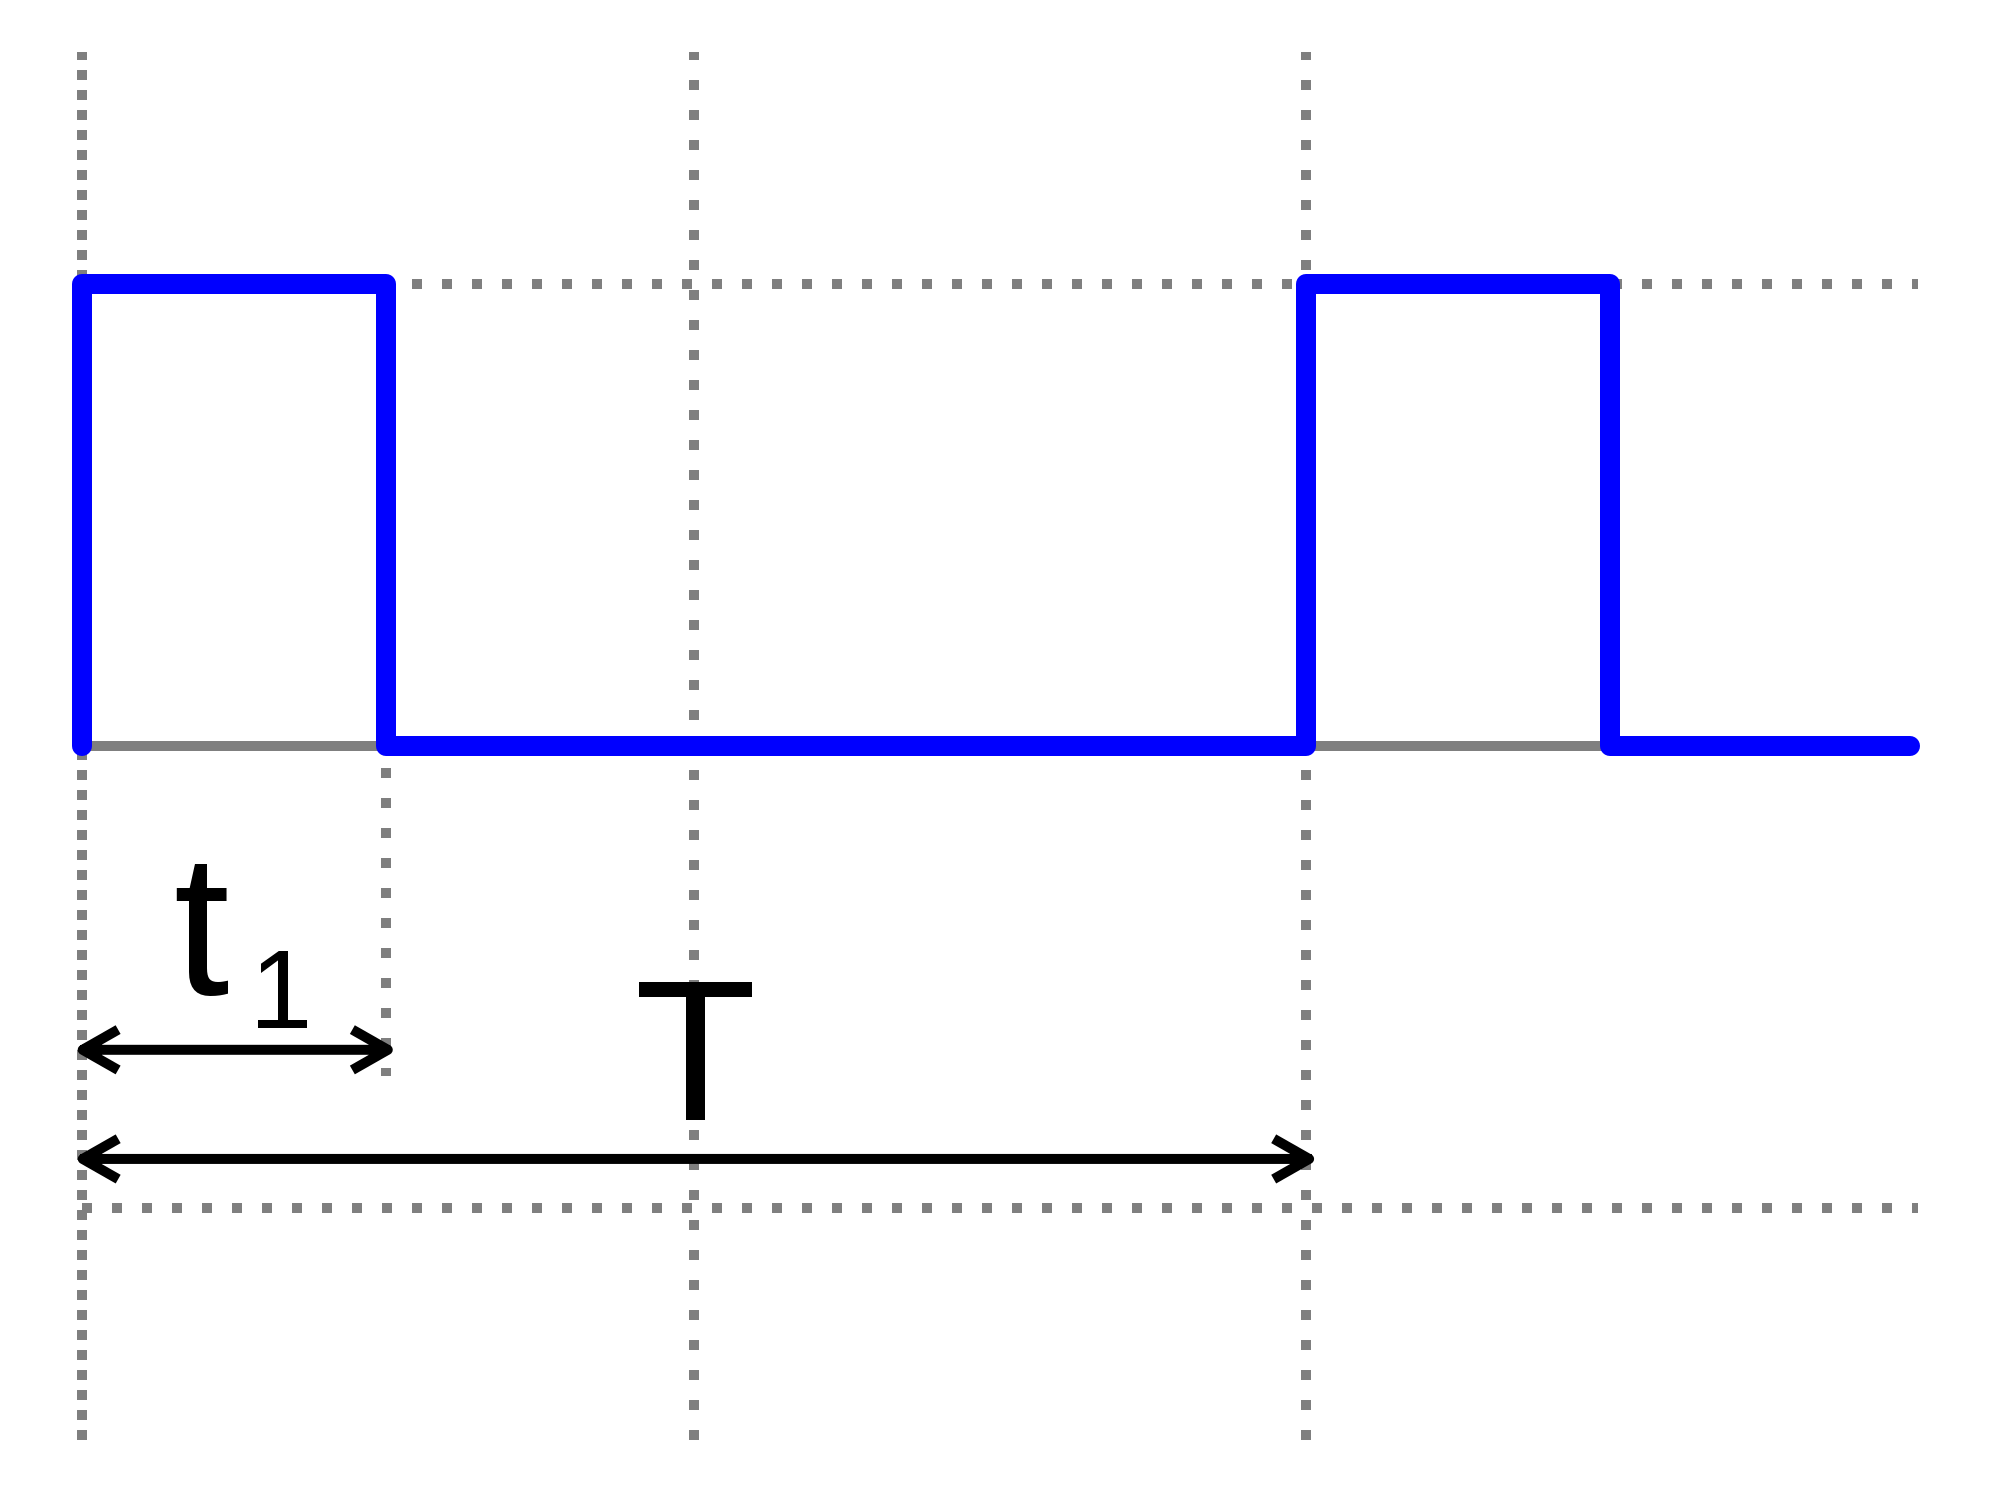
\includegraphics[width=2cm]{table/images/table_pulse_wide_wave.png} &
	&
	$\frac{t_1}{T}$ & $\sqrt{\frac{T}{t_1}}$ & $\sqrt{\frac{t_1}{T}}$ & $\sqrt{\frac{T}{t_1}}$ &
	$A\frac{t}{T}$ &
	$A^2\frac{t}{T}$ &
	$\frac{A^2t}{T}-\frac{A^2t^2}{T^2}$\\
\hline
\end{tabular}
\end{center}
\end{sidewaystable}

	